%%% The main file. It contains definitions of basic parameters and includes all other parts.

%% Settings for single-side (simplex) printing
% Margins: left 40mm, right 25mm, top and bottom 25mm
% (but beware, LaTeX adds 1in implicitly)
\documentclass[12pt,a4paper]{report}
\setlength\textwidth{145mm}
\setlength\textheight{247mm}
\setlength\oddsidemargin{15mm}
\setlength\evensidemargin{15mm}
\setlength\topmargin{0mm}
\setlength\headsep{0mm}
\setlength\headheight{0mm}
% \openright makes the following text appear on a right-hand page
\let\openright=\clearpage

%% Settings for two-sided (duplex) printing
% \documentclass[12pt,a4paper,twoside,openright]{report}
% \setlength\textwidth{145mm}
% \setlength\textheight{247mm}
% \setlength\oddsidemargin{14.2mm}
% \setlength\evensidemargin{0mm}
% \setlength\topmargin{0mm}
% \setlength\headsep{0mm}
% \setlength\headheight{0mm}
% \let\openright=\cleardoublepage

%% Generate PDF/A-2u
\usepackage[a-2u]{pdfx}

%% Character encoding: usually latin2, cp1250 or utf8:
\usepackage[utf8]{inputenc}

%% Prefer Latin Modern fonts
\usepackage{lmodern}

%% Further useful packages (included in most LaTeX distributions)
\usepackage{amsmath}        % extensions for typesetting of math
\usepackage{amsfonts}       % math fonts
\usepackage{amsthm}         % theorems, definitions, etc.
\usepackage{bbding}         % various symbols (squares, asterisks, scissors, ...)
\usepackage{bm}             % boldface symbols (\bm)
\usepackage{graphicx}       % embedding of pictures
\usepackage{fancyvrb}       % improved verbatim environment
\usepackage{natbib}         % citation style AUTHOR (YEAR), or AUTHOR [NUMBER]
\usepackage[nottoc]{tocbibind} % makes sure that bibliography and the lists
			    % of figures/tables are included in the table
			    % of contents
\usepackage{dcolumn}        % improved alignment of table columns
\usepackage{booktabs}       % improved horizontal lines in tables
\usepackage{paralist}       % improved enumerate and itemize
\usepackage{xcolor}         % typesetting in color

%%% Basic information on the thesis

% Thesis title in English (exactly as in the formal assignment)
\def\ThesisTitle{Deep-learning architectures for analysing population neural data}

% Author of the thesis
\def\ThesisAuthor{Petr Houška}

% Year when the thesis is submitted
\def\YearSubmitted{2021}

% Name of the department or institute, where the work was officially assigned
% (according to the Organizational Structure of MFF UK in English,
% or a full name of a department outside MFF)
\def\Department{Department of Software and Computer Science Education}

% Is it a department (katedra), or an institute (ústav)?
\def\DeptType{Department}

% Thesis supervisor: name, surname and titles
\def\Supervisor{Mgr. Ján Antolík, Ph.D.}

% Supervisor's department (again according to Organizational structure of MFF)
\def\SupervisorsDepartment{Department of Software and Computer Science Education}

% Study programme and specialization
\def\StudyProgramme{Computer Science}
\def\StudyBranch{Artificial Intelligence}

% An optional dedication: you can thank whomever you wish (your supervisor,
% consultant, a person who lent the software, etc.)
\def\Dedication{%
First and foremost, I'd like to thank my supervisor Mgr. Ján Antolík, Ph.D. for inviting me to a field that was entirely foreign to me at the beginning, providing thorough and ever-friendly guidance along the (not so short) journey. On a similar note, I want to express my deep gratitude to Prof. Daniel A. Butts for his invaluable and incredibly welcoming consultations regarding both the NDN3 library and the field of computational neuroscience in general.

Although I didn't end up doing my thesis under his supervision, RNDr. Milan Straka, Ph.D. deserves recognition for patiently lending me his valuable time while I was trying to figure out my eventual thesis topic.

Last but not least, I want to acknowledge at least some of the people who were, albeit indirectly, instrumental to me finishing this thesis. Be it through friendly nudging, emotional support, or even just being explicitly busy with their work and thus shaming me out of procrastination. In atmospherically random order, thank you: Václav \& Marcela Houškovi, Petra Millarová, Tomáš Thon, Eliška Kopecká, Ondřej Trhoň, and Adéla Syrová.
}

% Abstract (recommended length around 80-200 words; this is not a copy of your thesis assignment!)
\def\Abstract{%
Accurate models of visual system are key for understanding how our brains process visual information. In recent years, DNNs have been rapidly gaining traction in this domain. However, only few studies attempted to incorporate known anatomical properties of visual system into standard DNN architectures adapted from the general machine learning field, to improve their interpretability and performance on visual data.

In this thesis, we optimize a recent biologically inspired deep learning architecture designed for analysis of population data recorded from mammalian primary visual cortex when presented with natural images as stimuli. We reimplement this prior modeling in existing neuroscience focused deep learning framework NDN3 and assess it in terms of stability and sensitivity to hyperparameters and architecture fine-tuning. We proceed to extend the model with components of various DNN models, analysing novel combinations and techniques from classical computer vision deep learning, comparing their effectiveness against the bio-inspired components. 

We were able to identify modifications that greatly increase the stability of the model while securing moderate improvement in overall performance. Furthermore, we document the importance of small hyperparameters adjustments versus architectural advantages that could facilitate further experiments with the examined architectures. All-new model components were contributed to the open-source NDN3 package. 

Overall, this work grounds previous bio-inspired DNN architectures in the modern NDN3 environment, identifying optimal hyper-parametrization of the model, and thus paving path towards future development of these bio-inspired architectures.
}

% 3 to 5 keywords (recommended), each enclosed in curly braces
\def\Keywords{%
{deep-learning}, {computational neuroscience}, {v1 modeling}, {bio-inspired architectures}, {visual computation}
}

%% The hyperref package for clickable links in PDF and also for storing
%% metadata to PDF (including the table of contents).
%% Most settings are pre-set by the pdfx package.
\hypersetup{unicode}
\hypersetup{breaklinks=true}

% Definitions of macros (see description inside)
%%% This file contains definitions of various useful macros and environments %%%
%%% Please add more macros here instead of cluttering other files with them. %%%

%%% Minor tweaks of style

% These macros employ a little dirty trick to convince LaTeX to typeset
% chapter headings sanely, without lots of empty space above them.
% Feel free to ignore.
\makeatletter
\def\@makechapterhead#1{
  {\parindent \z@ \raggedright \normalfont
   \Huge\bfseries \thechapter. #1
   \par\nobreak
   \vskip 20\p@
}}
\def\@makeschapterhead#1{
  {\parindent \z@ \raggedright \normalfont
   \Huge\bfseries #1
   \par\nobreak
   \vskip 20\p@
}}
\makeatother

% This macro defines a chapter, which is not numbered, but is included
% in the table of contents.
\def\chapwithtoc#1{
\chapter*{#1}
\addcontentsline{toc}{chapter}{#1}
}

% Draw black "slugs" whenever a line overflows, so that we can spot it easily.
\overfullrule=1mm

%%% Macros for definitions, theorems, claims, examples, ... (requires amsthm package)

\theoremstyle{plain}
\newtheorem{thm}{Theorem}
\newtheorem{lemma}[thm]{Lemma}
\newtheorem{claim}[thm]{Claim}

\theoremstyle{plain}
\newtheorem{defn}{Definition}

\theoremstyle{remark}
\newtheorem*{cor}{Corollary}
\newtheorem*{rem}{Remark}
\newtheorem*{example}{Example}

%%% An environment for proofs

\newenvironment{myproof}{
  \par\medskip\noindent
  \textit{Proof}.
}{
\newline
\rightline{$\qedsymbol$}
}

%%% An environment for typesetting of program code and input/output
%%% of programs. (Requires the fancyvrb package -- fancy verbatim.)

\DefineVerbatimEnvironment{code}{Verbatim}{fontsize=\small, frame=single}

%%% The field of all real and natural numbers
\newcommand{\R}{\mathbb{R}}
\newcommand{\N}{\mathbb{N}}

%%% Useful operators for statistics and probability
\DeclareMathOperator{\pr}{\textsf{P}}
\DeclareMathOperator{\E}{\textsf{E}\,}
\DeclareMathOperator{\var}{\textrm{var}}
\DeclareMathOperator{\sd}{\textrm{sd}}

%%% Transposition of a vector/matrix
\newcommand{\T}[1]{#1^\top}

%%% Various math goodies
\newcommand{\goto}{\rightarrow}
\newcommand{\gotop}{\stackrel{P}{\longrightarrow}}
\newcommand{\maon}[1]{o(n^{#1})}
\newcommand{\abs}[1]{\left|{#1}\right|}
\newcommand{\dint}{\int_0^\tau\!\!\int_0^\tau}
\newcommand{\isqr}[1]{\frac{1}{\sqrt{#1}}}

%%% Various table goodies
\newcommand{\pulrad}[1]{\raisebox{1.5ex}[0pt]{#1}}
\newcommand{\mc}[1]{\multicolumn{1}{c}{#1}}

%%% Ref helpers
\newcommand{\refsection}[1]{\textit{\nameref{#1}} (section \ref{#1})}
\newcommand{\refattachment}[1]{\texttt{\nameref{#1}} (attachment \ref{#1})}

\newcommand{\tttnameref}[1]{\texttt{\nameref{#1}}}


% Title page and various mandatory informational pages
\begin{document}
%%% Title page of the thesis and other mandatory pages

%%% Title page of the thesis

\pagestyle{empty}
\hypersetup{pageanchor=false}
\begin{center}

\centerline{\mbox{
\includegraphics[width=166mm]{../img/logo-en.pdf}}}

\vspace{-8mm}
\vfill

{\bf\Large MASTER THESIS}

\vfill

{\LARGE\ThesisAuthor}

\vspace{15mm}

{\LARGE\bfseries\ThesisTitle}

\vfill

\Department

\vfill

{
\centerline{\vbox{\halign{\hbox to 0.45\hsize{\hfil #}&\hskip 0.5em\parbox[t]{0.45\hsize}{\raggedright #}\cr
Supervisor of the master thesis:&\Supervisor \cr
\noalign{\vspace{2mm}}
Study programme:&\StudyProgramme \cr
\noalign{\vspace{2mm}}
Study branch:&\StudyBranch \cr
}}}}

\vfill

% Zde doplňte rok
Prague \YearSubmitted

\end{center}

\newpage

%%% Here should be a bound sheet included -- a signed copy of the "master
%%% thesis assignment". This assignment is NOT a part of the electronic
%%% version of the thesis. DO NOT SCAN.

%%% A page with a solemn declaration to the master thesis

\openright
\hypersetup{pageanchor=true}
\pagestyle{plain}
\pagenumbering{roman}
\vglue 0pt plus 1fill

\noindent
I declare that I carried out this master thesis independently, and only with the cited
sources, literature and other professional sources. It has not been used to obtain another
or the same degree.

\medskip\noindent
I understand that my work relates to the rights and obligations under the Act No.~121/2000 Sb.,
the Copyright Act, as amended, in particular the fact that the Charles
University has the right to conclude a license agreement on the use of this
work as a school work pursuant to Section 60 subsection 1 of the Copyright~Act.

\vspace{10mm}

\hbox{\hbox to 0.5\hsize{%
In \hbox to 6em{\dotfill} date \hbox to 6em{\dotfill}
\hss}\hbox to 0.5\hsize{\dotfill\quad}}
\smallskip
\hbox{\hbox to 0.5\hsize{}\hbox to 0.5\hsize{\hfil Author's signature\hfil}}

\vspace{20mm}
\newpage

%%% Dedication

\openright

\noindent
\Dedication

\newpage

%%% Mandatory information page of the thesis

\openright

\vbox to 0.5\vsize{
\setlength\parindent{0mm}
\setlength\parskip{5mm}

Title:
\ThesisTitle

Author:
\ThesisAuthor

\DeptType:
\Department

Supervisor:
\Supervisor, \SupervisorsDepartment

Abstract:
\Abstract

Keywords:
\Keywords

\vss}

\newpage

\openright
\pagestyle{plain}
\pagenumbering{arabic}
\setcounter{page}{1}


%%% A page with automatically generated table of contents of the master thesis

\tableofcontents

%%% Each chapter is kept in a separate file
\chapter*{Introduction}
\addcontentsline{toc}{chapter}{Introduction}

\section*{History \& context}
\addcontentsline{toc}{section}{History \& context}
According to the annals of history, the term \textit{computational neuroscience} was coined by Eric L. Schwartz in 1985 when he organized a conference\footnote{\citep{schwartz1990computational}} to provide a summary of the current status of a field at that time known under a variety of names such as neural modeling, brain theory, and neural networks. The central idea of computational neuroscience, to study the brain through mathematical models, is much older than that, however. First modern traces can be found as early as in 1907 when Louis Lapicque introduced\footnote{\citep{Lapicque1907}} the integrate and fire model. While crude, the model managed to describe observed interactions of a nerve fiber long before the exact mechanisms responsible for generation of neuron action potentials were discovered. Doing so, it greatly contributed to our understanding of the brain and laid a strong foundation for further research.

One of the main approaches in computational neuroscience goes under the name \textit{system identification}: first, through experimentation one obtains a large dataset of input and output pairs of a given neural system - e.g. pairs of images and responses of neurons in primary visual cortex. These are subsequently fitted through machine learning methods with a model, in the hope of identifying the computations that the neural system does to translate the inputs to its outputs. 

Such methods effectively enable us to predict the response of a system to an arbitrary plausible input. Doing so is one of the best ways to test our understanding of such a system. While having a model that predicts the response accurately does not necessarily have to mean our understanding of the biological fundamentals is correct, it is a clear signal it is at least plausible. On the other hand, the opposite, when a model based on our knowledge is not accurate, is proof we should revisit our assumptions. Such an approach is particularly effective in early stages of sensory systems whose primary function is to produce a response encoding to a clearly defined input - sensory stimulus. 

Unsurprisingly, going as far back as to the 1960s, visual neuroscience has been close to traditional image processing and has used its toolkit for computational modeling. The influence was not one-sided. Several ideas, such as convolution layers, inspired by biological observations\footnote{\citep{Lindsay_2020}} have found their way back to classical computer vision. In recent years, the combination of advancements in deep learning vision and higher volume of better data in visual neuroscience, have caused increased focus on deep learning inspired neural models. 

Deep learning inspired models are only a rough approximation of biological reality, not only at the level of single neuron biophysics but also in terms of overall network architecture. For example, deep neural network (DNN) architectures typically do not model interactions between neurons within a single layer or do not account for direct nonlinear interactions between neurons, such as those provided by neuromodulation or attentional mechanisms in the biological brain. 

\section*{Motivation}
\addcontentsline{toc}{section}{Motivation}
Regardless, classic DNNs are still immensely useful. Through the ability to fit their many parameters to real data, and access to ever increasing toolkit of high performance methods borrowed from classical machine learning, they allow for effective means of approximating the stimulus-response function in many neural subsystems. And thanks to their abstraction level, rapid experimentation of higher level concepts is also easier. Much like the integrate and fire model that also abstracted over certain details, they can still inform our understanding of the nature of vision processing. 

However, despite the success of DNNs in neuroscience, having outclassed classical system identification methods in most domains, there remains a substantial gap between the predictions these models give and the actual measured neural responses. This is true even in the most peripheral stages of visual processing such as primary visual cortex. Furthermore, the poor interpretability of the DNN models has been identified as a major challenge limiting their usefulness for understanding neural computation.

To address these issues, a recent model by \cite{antolik}, which will be the focus of the present thesis, explored the idea of incorporating more biologically plausible components into the DNN framework. It showed that such an approach leads to a model with fewer parameters, better interpretability, and outperformed, at the time of writing, other state-of-the-art approaches. 

However, the \citeauthor{antolik} \citeyear{antolik} study also showed shortcomings. The model was very sensitive to random initialization, most hyper-parameters of the model were not thoroughly studied, and more direct one-to-one comparison of the biologically inspired versus classical DNN components was missing. Furthermore, since its publishing, several studies using classical DNN techniques managed to demonstrate slight improvement over the \citeauthor{antolik} data. Finally, the model has been implemented in an ad-hoc way in now discontinued ML framework Theano, which poses a problem for further exploration of the bio-inspired DNNs architecture idea.

\section*{Motivation}
\addcontentsline{toc}{section}{Motivation}
The goal of this thesis is to address the outlined outstanding issues with the \citeauthor{antolik} study, in order to provide a stable, fine-tuned, and well characterized implementation in a modern neuroscience oriented DNN framework to enable future experimentation with this bio-inspired architecture. Following contributions are the goals of this thesis:

\begin{itemize}
    \item \textbf{Assess the \citeauthor{antolik} model (and its variants) in terms of stability and sensitivity to hyperparameter finetuning:} Especially on low quantities of noisy data, which is common in the field of sensory neuroscience, models tend to be relatively unstable with respect to both hyperparameters fine-tuning but also random initialization. We want to quantify the effects and hopefully explore ways to mitigate them to ensure any conclusions drawn are not due to a chance but rather architectural properties. As part of this, we will make use of our whole dataset, comparing various architectures across its three separate subsets.
    \item \textbf{Evaluate novel architectures inspired by classical computer vision:} We want to compare the benefits of biologically restricted techniques with more computationally generic approaches from classical deep computer vision and investigate whether hard constraints could be replaced with well chosen regularization schemes. Furthermore, test the impact of several deep learning techniques that were shown to work on classical computer vision problems.
    \item \textbf{Improve upon \citeauthor{antolik} model:} Decrease the gap between the original model and more recent less biologically constrained architectures that demonstrated improved performance. 
    \item \textbf{Contribute new functionality to the NDN3 library toolbox:} We contribute all tools developed to conduct experiments in this thesis upstream to the NDN3 framework or, where not applicable, publish them separately under open source license. The goal is to enable others to iterate on our findings and evaluate the results in a shared environment.
    \item \textbf{(Re)implement and assess the \citeauthor{antolik} model and several of its variants within the NDN3 framework:} Similar to the previous point, implementing and analysing various models within a shared framework aims to enable rapid prototyping, and generally facilitate further research.
    \item \textbf{Identify opportunities for further research:} Since our set of goals is relatively broad, we will not be able to dive deep into every encountered question. As a result, we want to identify opportunities for more focused further research.
\end{itemize}

This way, the present thesis represents a stepping stone that will accelerate the future long-term research program on bio-inspired DNN architectures for neuroscientific data underway in the \citeauthor{antolik} group.

\section*{Thesis structure}
\addcontentsline{toc}{section}{Thesis structure}
This thesis is divided into 4 parts. First, in \hyperref[ch:1]{chapter 1} we provide the theoretical background. We start with a high level overview of the initial part of the visual processing system. Then, we introduce both computational neuroscience generally and the tools it uses for system identification tasks, as well as provide a brief summary of the deep learning techniques that will be relevant for our experiments. In \hyperref[ch:2]{chapter 2}, we introduce the \citeauthor{antolik} model and other especially relevant work in more detail. Second, in chapters \hyperref[ch:3]{chapter 3} we describe the implementation of the additional methods necessary to realize our architectures and the experiments pipeline. Then, in \hyperref[ch:4]{chapter 4}, we introduce our methodology for both the model exploration and results analysis, and finish with a training regime overview.

\hyperref[ch:5]{Chapter 5} with experiments and their results follows. We start by reimplementing the \citeauthor{antolik} model. In the first section, we analyse it in terms of stability and sensitivity to training hyperparameters, attempting to get the best and most stable version possible. Then we test regularization on the fully connected layers, impact of additional non-linearity, and input scaling. In the second section, we move towards larger architectural changes, testing elements from other state of the art models, traditional deep computer vision, but also drawing inspiration from simpler tools of computational neuroscience. We conduct a comparison between various computationally similar architectures differing only by the explicitness of imposed regularization. In the third section we explored the effects of transfer learning, by training one instance of a model on all of the dataset’s three separate subsets pooled together. Further, we train the best variants of architectures from previous sections and compare their results to assess the universality of their improvements.

Finally, the last \hyperref[ch:6]{chapter} offers a summary of our findings, provides lessons learned, and suggests ample opportunities for further research.
\chapter{Background}\label{ch:1}

\section{Visual sensory neuroscience}
In this section, we provide an introduction to visual neuroscience necessary for understanding the biological plausibility of our models. For a more comprehensive and in-depth introduction to neuroscience of vision please refer to \textit{Neuroscience: Exploring the Brain} \citep{bear_neuroscience:_2007} or the excellent summary provided as part of \cite{Carandini10577}'s review.

\subsection{Early visual system}\label{ch:1.1.1}
In this thesis we restrict our focus to the first 3 early stages of visual processing, corresponding to three neural structures: the retina, lateral geniculate body (LGN) and primary visual cortex (V1).

The journey of a visual stimuli starts on the retina at the back of an eye, where photosensitive cells - rods and cones measure the intensity of the light reflected by objects in our field of vision and projected at the back of our eye by cornea. While the particularities of rods and cones are interesting, especially when it comes to color processing, for the purpose of this introduction we will treat them as simple detectors that output electrical signal proportional to the sensed luminance, resulting in what could be abstracted as a matrix of luminescence levels - a raster image. 

The first processing step happens directly in the eye through retinal ganglion cells. Again, these cells are more complicated than presented here, but on a high level they detect local features such as contrast, directional movement of small stimuli, etc. The two main types are ON and OFF cells, both having a circular receptive field. Receptive field is the portion of sensory space that elicits neural responses when stimulated. In case of vision that means the section of the visual field a particular neuron responds to. ON cells fire when a high luminance hits the the center of its receptive fields and the disk at the edge is, proportionally, less excited. OFF cells function in the exact opposite way. For illustration, refer to figure \ref{fig:1.1}.

\begin{figure}
    \centering
    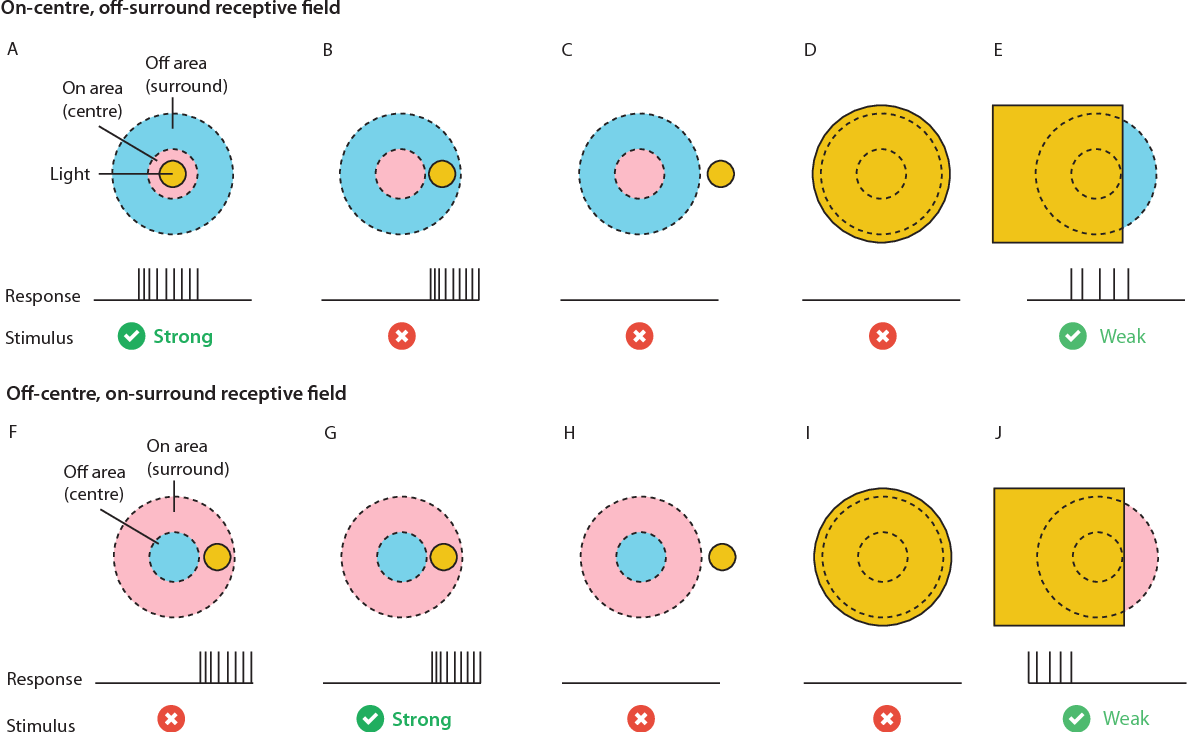
\includegraphics[width=1\textwidth]{../figures/01_33-Figure2.8-1}
    \caption[Receptive fields of retinal ganglion and LGN cells]{Receptive fields of retinal ganglion and LGN cells. Adapted from \citep{thesis_2015}.}
    \label{fig:1.1}
\end{figure}

From the eye most of the signal travels to LGN\footnote{Describing the visual pathway as a strictly feed-forward network is a great simplification.}, which serves as an active bridge to the visual cortex at the back side of the brain. Much like later V1, LGN is composed of 6 layers. The processing that happens here could be summarized as very similar to the retinal ganglion cells, only with bigger receptive fields. It is important to note that LGN does not get input only or even mainly from retina. It also receives substantial feedback from the primary visual cortex, and has synapses from parts of the thalamus and the brain stem. For example, the brain stem connection is believed to be responsible for perceived visual impacts of alertness changes, such as a flash of light when one is startled in a dark room. However, the exact role of these extra-retina sources in LGN function remains largely not understood. This means that the activity of both LGN, and all downstream stages of processing, such as V1, is modulated not only by the visual stimuli but also other neural activity inducing factors, for example emotions, locomotion, or other sensory inputs. Any models predicting the activity of LGN, V1, or higher stages of visual processing that are based solely on visual stimuli cannot, therefore, explain the entirety of recorded data. Nevertheless, under restricted experimental conditions, a wide range of studies have shown that the response of LGN cells can be very well approximated by a linear filter composed of difference-of-Gaussians. 

At last, the signal reaches the primary visual cortex. It is divided into 6 layers. Within V1, we recognize two main functional cell types - the so-called simple and complex cells. Simple cells, as their name suggests, can be represented as mostly linear combinations of ON and OFF cells. This means that within their receptive fields, they have well defined excitatory and inhibitory regions. In essence, they elicit response when stimulus, in this case light, hits the excitatory regions substantially more than the inhibitory regions. Their receptive field tends to be axis aligned, making them sensitive to oriented edges and gratings. They are also commonly described as Gabor-like filters (see Fig. \ref{fig:1.2}). 

\begin{figure}[H]
    \centering
    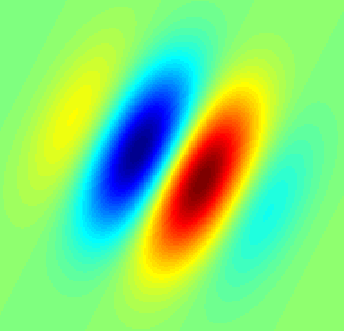
\includegraphics[width=0.2525\textwidth]{../figures/01_Gabor_filter}
    \caption[Gabor filter-type receptive field typical for a simple cell]{Gabor filter-type receptive field typical for a simple cell. Blue regions indicate inhibition, red excitation. Figure was adopted from \citep{pict_gabor_filter}.}
    \label{fig:1.2}
\end{figure}

The nature of complex cells is not yet entirely settled, but it is understood that the relationship between the visual input and their response cannot be explained with linear function. Complex cells are known to be orientation selective, just as their simple counterparts, but their hallmark is that they are not sensitive to the exact position of the oriented stimulus within their receptive field. It is thus hypothesized that their output is a non-linear combination of a number of co-oriented simple cells. If the hypothesis was true, it would essentially create a hierarchy, where the LGN cells roughly correspond to concentric ON/OFF filters of the stimuli, simple cells to a linear combination of LGN neurons, and complex cells to nonlinear combinations of simple cells. In addition to aforementioned stimuli, V1 neurons are also selective to other visual features, such as color, phase, spatial and temporal frequencies etc.

\section{Computational neuroscience}

In the following subsections, we provide an introduction to the traditional system identification methods used in visual neuroscience. For further details, refer to \textit{Data-driven approaches to understanding visual neuron activity} \citep{doi:10.1146/annurev-vision-091718-014731} or \cite{Carandini10577}'s review.

\subsection{General overview}

In computational neuroscience, we can generally distinguish two lines of inquiry. The first one, attempts to model biological reality even on the lowest level, focusing on particularities of every single neuron. Due to the inherent computational requirements of evaluating the biological neuron model, including the necessity to properly simulate temporarily to allow for mechanisms like refractory period, they usually do not scale well to larger systems. Such models are usually too complex, with too many free parameters to be fitted directly to recorded neural data through gradient based techniques. 

The second approach abstracts away details of singular neurons and focuses on higher level computation and topological properties. As such, it can leverage tools from classical machine learning and most recently even deep learning. It is prevalent in visual sensory neuroscience where it is commonly needed to model ‘black-box’ systems, such as the whole path from retina to primary visual cortex across dozens of neurons. In such models, the neural function is represented by a relatively generic computation whose parameters are fit to data to correspond to each neuron’s specific processing. Formally, for stimuli $s$, response $r$, parameters (also called weights) $o$, and model $m$, we have (Eq. \ref{eq:1.1}).

\begin{equation}\label{eq:1.1}
    r=m(s|o)
\end{equation}

In the rest of this chapter, and thesis in general, we will consider only statistical models for solving system identification tasks within the domain of visual sensory neuroscience. Our inputs will be images presented to a subject, in case of our data a mouse, in a form of 2D pixel matrices. The outputs will be real values, one per recorded neuron, representing an estimate of the measured neural activity elicited by presentation of the given image.

\subsection{Classical models}\label{ch:1.2.2}
The simplest method possible for predicting a single neuron’s response to an image stimuli is a linear model, essentially a linear regression over the pixels of the input. Mathematically, for parameters $o$ (also called weights, or in this case filter) and an image of height $h$ and width $w$ pixels that gives us the equation \ref{eq:1.2}. In such a linear model, the weights can be fitted in a number of ways, either through gradient descent methods, or analytically to compute the optimal solutions from the whole dataset. The second approach is commonly called Spike Triggered Average (STA). Both ways of fitting can incorporate regularization for the weights, for example to punish a high first derivative in both spatial dimensions, ensuring smoothness \citep{first_kernel}. This is particularly necessary in the neuroscientific settings where datasets tend to be of limited size, and overfitting of models is thus a major challenge. 

\begin{equation}\label{eq:1.2}
    r = \sum_{x,y=0}^{w,h} s_{x,y} * o_{x,y}
\end{equation}

A natural extension of a linear model is a linear-nonlinear (LN) model. As the name suggests, it is a linear model whose output is modulated by a single nonlinear function $f$ (Eq. \ref{eq:1.3}). This type of model is commonly used in a regularized variant (rLN). Due to its direct interpretability - we can easily visualise the filter, ease of analysis - the parameters (filters) are easy to compare and work with using image processing toolkit, and computational simplicity - it is just a linear operation, LN models were the de facto standard model of computational neuroscience until relatively recently.

\begin{equation}\label{eq:1.3}
    r = f(s \cdot o)
\end{equation}

In an effort to further improve the prediction power of the LN model, several of its extensions appeared. First as a generalized LN model (GLM), where one filter is replaced with a set of $k$ filters (Eq. \ref{eq:1.4}). 

\begin{equation}\label{eq:1.4}
    r = f(s \cdot o_0, s \cdot o_1, ..., s \cdot o_k)
\end{equation}

Since the k-ary non-linearity function can combine the individual results in a non-linear way, this increases the computational expressiveness of the model. There are two limitations of this approach. It makes the k-ary function an additional hyperparameter and, in turn, does not allow the way individual filters are combined to be fitted to data. The LNLN model solves both problems, replacing the k-ary non-linear function with a linear combination of several LN models (Eq. \ref{eq:1.5}):

\begin{equation}\label{eq:1.5}
    r = f(\sum_{i=0}^{k} w_i * f_i(s \cdot o_i))
\end{equation}

In addition to solving the two problems of GLM and being more interpretable, as it is simply a linear combination of LN models whose filters we can visualise with a non-linearity at the end, the fact that the combination can be individually parametrized opened the door to a particular multi-step learning strategy. When modeling multiple neurons that are believed to be similar in function, we can share the first level filters ($o_i$) between them, and only individually fit the $w$ parameters. This allows the filters $o_i$ to be based on more data - from all neurons instead of just one, and in turn, decreases the chance for overfitting.

\label{intr:hard-reg}\label{intr:soft-reg}Furthermore, the filters can be parametric, e.g. gabor functions \citep{Kay2008}, gaussians, or pre-computed bank of filters - for example borrowed from classical image processing toolkit. This can serve two goals. First, significantly decrease the number of free parameters of the model. While a normal filter for a 31x31 image has 961 parameters, a simple gaussian filter has only 4, strength, x and y coordinates of the center, and width. Second, it can ground the model in biological reality. For example, the computational properties of retinal ganglion cells are known to be well approximated in space by a difference-of-Gaussian function\footnote{A subtraction of two concentric 2D Gaussians.} and so one can inject such priors in the model. We will call this approach hard regularization. Similar effect can be achieved on arbitrary filters with regularization during parameter fitting which penalizes forms of the filter that diverge from our desired shape, as explained above for the LN model. We will call that soft regularization.

\section{ML and Deep neural networks}
In this section we will provide a brief overview of deep neural networks (DNN) fundamentals to introduce the most relevant principles and unite terminology. For a comprehensive description of general machine learning and particularly DNN methods please refer to the \textit{Deep Learning book} \citep{Goodfellow-et-al-2016}.

\subsection{Feed forward neural network}
Deep neural network (DNN) is a statistical machine learning model vaguely inspired by the brain. The term neural comes from the fact that it is traditionally composed of computational neurons\footnote{Not to be confused with biological neurons.} (also called perceptrons\footnote{\citep{Rosenblatt1958ThePA}}). Computational neurons are mathematically defined as a weighted sum of their inputs followed by, usually a non-linear, activation function. Deep and networks, because they are usually composed of several interconnected layers of neurons. A single layer of a DNN is defined by its inputs $x$ and outputs $y$ tensors. The output of the $k$-th neuron of the simplest, a fully connected, layer with $n$ inputs is then (Eq. \ref{eq:1.6}):

\begin{equation}\label{eq:1.6}
    y_k = f(\sum_{i}^{n} x_{i} * w_{k,i})
\end{equation}

When multiple layers $f_1, f_2, \dots, f_n$ are stacked on each other - to form a deep neural network, the outputs of the preceding layer are used as the inputs of the following one. The output of a complete DNN is then $y = f_n(\dots f_2(f_1(x))\dots)$. To tie this back to computational neuroscience, a LN model would be a single layer neural network. Its input size would be equal to the size of stimulus and output size to 1, as we are predicting a single neuron. Similarly, a single neuron LNLN model would be two layers DNN, where the size of the first layer would correspond to the number of LNLN filters, and the second would have size 1. If we wanted a LNLN model where the filters are shared across multiple fitted neurons, it would again be two layers DNN. The second layer would have size corresponding to the number of recorded neurons, however. Each output neuron (output of the second layer) would then be an independent combination of shared filters (the outputs of the first layer).

\begin{table}[h]
    \renewcommand{\arraystretch}{1.2}
    \centering
    \begin{tabular}{l|l}
        \toprule
        \textbf{Name} & \textbf{Function} \\ \midrule
        ReLU & $f(x) = max(0, x)$ \\ 
        Sigmoid & $f(x) = \frac{1 }{1 + e^{-x} } $ \\ 
        SoftPlus & $f(x) = ln(1+e^x)$ \\ 
        Linear/Identity & $f(x) = x$ \\ 
        TanH & $f(x) = tanh(x)$ \\ \bottomrule

    \end{tabular}
    \caption[Commonly used activation functions]{Some of the commonly used activation functions\protect\footnotemark.}
    \label{tab:1.1}
    \renewcommand{\arraystretch}{1.0}
\end{table}

\footnotetext{For neural modeling, strictly positive functions such as ReLU or SoftPlus are especially interesting due to the non-negative nature of firing rate.}

Much like the LNLN filters, DNN layers do not have to be generic. Similar to what we termed hard regularization, they can exploit known properties of the computation they are trying to model. Most notably, convolutional layers make use of local properties of inputs with continuous dimensions, such as the spatial dimensions of image inputs\footnote{Deep neural networks with convolutional layers are commonly called convolutional neural networks (CNN).}. Their outputs are the result of a location invariant filter applied at all spatial locations of the input. For more information, refer to introduction to \textit{Convolutional networks} in \cite{thesis_hojdar}.

\subsection{DNN training}\label{ch:1.3.2}

Due to the number of free parameters in even relatively shallow DNNs, these models cannot be fitted analytically. Instead, iterative gradient descent based methods, such as stochastic gradient descent (SGD \citep{kiefer1952}) or more recently ADAM \citep{kingma2014adam}, are commonly used. In gross simplification, the fitting process, also called model training, works as follows. A small random subset (batch) of input and corresponding desired output (gold data) is taken from the dataset. The input portion of a batch is used as the model’s input, computation happens, and we get a prediction (response) from the model. Then, the model’s response and corresponding gold data are put into a loss function. It serves as the metric of how far the model prediction was from the desired output. The loss function can also penalize certain properties of the model’s parameters (e.g. increase the loss for every non-zero weight). As the last step, first derivatives of the loss function with respect to all the model’s free parameters are taken (gradient) and subtracted (model update) from the parameters to, in theory, decrease the loss value next time. This step is repeated for all batches in our dataset\footnote{This means a larger batch size proportionally leads to less model updates per epoch.}. The whole process up until now constitutes one epoch. Epochs are then repeated until convergence.

In addition to layers that provide direct computation, DNNs can also feature layers whose primary objective is to help during training. One such example is the dropout layer as introduced by \cite{JMLR:v15:srivastava14a}. It randomly zeros portion of its output neurons during training, thus forcing the rest of the network to not to rely on individual inputs, and prevents overfitting\footnote{Another interpretation of the dropout layer is that it effectively trains an ensemble of models that share the majority of parameters.}. Another is the batch normalisation layer introduced by \cite{2015arXiv150203167I}, that forces its outputs to be of 0 mean and 1 variance within a single batch, and - if needed - to learn any linear transformation of its outputs explicitly. This aims to stabilise the learning process. 

\subsection{Transfer learning}
Training a DNN, e.g. for a vision task, from scratch requires large amounts of data. Fortunately, the observation that the initial layers of any DNN trained on image data are functionally similar, starting at low-level feature detection and eventually building up to higher level concepts, allows us to leverage models trained on generic tasks with huge pre-existing datasets. 

We can simply take an initial portion of an already trained network, use its layers including trained weights as the foundation of a new model, and only append it with a few new problem specific layers that are then trained from scratch. This can substantially cut down on the amount of data required, as we only need to constrain the parameters of newly added layers, and also serves as a regularization technique, making sure the initial low level filters are not overfitted on our limited data\footnote{\citep{2018arXiv180801974T}}. 

\section{DNNs and computational neuroscience}
There are several differences between system identification tasks of computational neuroscience and classical problems of computer vision. Mainly, the amount and quality of data. Where for example image classification datasets usually feature tens of thousands of precisely annotated examples\footnote{Cifar-10: \citep{cifar10}, Fashion-MNIST: \citep{xiao2017}}, system identification tasks on early visual processing have often only few thousands of substantially noisy recordings. This has vast implications for not only viable architectures, as more layers mean more free parameters (e.g. 65 millions in case of YOLOv3\footnote{\citep{2018arXiv180402767R}}) that have to be constrained by data to prevent overfitting, but - as we will see, also has the potential to invalidate our intuition around many aspects such as regularization and model stability we might have from working with larger models and datasets. 

In the following section we will introduce particular tools and techniques that are commonly used by system identification methods in neuroscience and which will be featured in our exploration, but are not as well known in the classical machine learning or computer vision domain. 

\subsection{Poisson versus Gaussian loss function}\label{ch:1.4.1}

Since our system classification problem is essentially a regression, the output consists of a real valued response for each neuron. We need an appropriate loss function to measure the distance of the model’s prediction to the recorded data. It is common to assume that the data contains noise with Gaussian distribution and then construct the loss function through most likelihood estimation (MLE) method, leading to mean squared error (MSE). Gaussian distribution is commonly used due to it being the maximum entropy probability distribution for a fixed mean and standard deviation. Intuitively speaking, it is the distribution that assumes the least given mean, which is zero for the noise, and static variance.

In our case, with outputs that are proportional to the spike rates of neurons, we do not have to assume the most generic distribution, however. There is evidence \citep{Goris2014} that the variance of neural response roughly corresponds to the neuron’s firing rate. Furthemore, spiking outputs are strictly non-negative, invalidating the assumption of Gaussian distribution. That means Poisson distribution, which assumes variance proportional to its mean and is non-negative, is a more optimal choice for modeling them. Through MLE, for measured firing rate $x$ and predicted firing rate $y$ that gives us the loss function on equation \ref{eq:1.7} .

\begin{equation}\label{eq:1.7}
    loss(x,y)=y-x\log{(y)}
\end{equation}

\subsection{Correlation as performance metric}\label{ch:1.4.2}

Even though the loss function based on Poisson noise assumption is the optimal metric to optimise during training, it is not very good for eventual analysis and comparison of different models, potentially across multiple datasets. Not only is it dependent on the assumed noise distribution, which is a technical detail of the fitting process, rather than a feature of the actual resulting fitted model, but it is also influenced by the scale of output data, and generally does not have an intuitive interpretation.

For those reasons, either the Pearson’s correlation coefficient (Eq. \ref{eq:1.8}) or the proportion of explained variance between each neuron’s model predicted output and its measured response is more commonly used instead. In this thesis, we will use Pearson’s correlation coefficient averaged across all recorded neurons for simplicity.

\begin{equation}\label{eq:1.8}
r(x, y) = \frac{{}\sum_{i=1}^{n} (x_i - \overline{x})(y_i - \overline{y})}
{\sqrt{\sum_{i=1}^{n} (x_i - \overline{x})^2(y_i - \overline{y})^2}}
\end{equation}

\subsection{Regularizations}
In addition to the wide set of traditional parameters regularizations common to all machine learning methods, such as L1 and L2, that simply punish either the size of or the number of non-zero parameters, computational neuroscience commonly uses regularizations inspired by biological plausibility. One such regularization, that will be prominent in our experiments, is Laplacian regularization, an L2 penalty on a Laplacian convolution filter. By punishing high first order derivatives in spatial dimensions, it ensures smoothness of regularized filters.

\begin{table}[h]
    \renewcommand{\arraystretch}{1.2}
    \centering
    \begin{tabular}{l|l}
        \toprule
        \textbf{Name} & \textbf{Function} \\ \midrule
        L1 & $\sum_i \abs{|w_i|}$ \\ 
        L2 & $\sum_i w_i^2$ \\ 
        Laplacian & $\sum_{x,y, i, o}(W_{:,:, i, o}*L)_{x,y}^2, \quad L=\left[\begin{smallmatrix}
0 & 1 & 0\\
1 & -4 & 1\\
0 & 1 & 0\end{smallmatrix}\right]$
 \\ \bottomrule
    \end{tabular}
    \caption[Relevant weights soft regularizations.]{Relevant weights soft regularizations.}
    \label{tab:1.2}
    \renewcommand{\arraystretch}{1.0}
\end{table}

\chapter*{Conclusion}
\addcontentsline{toc}{chapter}{Conclusion}


%%% Bibliography
%%% Bibliography (literature used as a source)
%%%
%%% We employ bibTeX to construct the bibliography. It processes
%%% citations in the text (e.g., the \cite{...} macro) and looks up
%%% relevant entries in the bibliography.bib file.
%%%
%%% The \bibliographystyle command selects, which style will be used
%%% for references from the text. The argument in curly brackets is
%%% the name of the corresponding style file (*.bst). Both styles
%%% mentioned in this template are included in LaTeX distributions.

\bibliographystyle{plainnat}    %% Author (year)
% \bibliographystyle{unsrt}     %% [number]

\renewcommand{\bibname}{Bibliography}

%%% Generate the bibliography. Beware that if you cited no works,
%%% the empty list will be omitted completely.

\bibliography{bibliography}

%%% If case you prefer to write the bibliography manually (without bibTeX),
%%% you can use the following. Please follow the ISO 690 standard and
%%% citation conventions of your field of research.

% \begin{thebibliography}{99}
%
% \bibitem{lamport94}
%   {\sc Lamport,} Leslie.
%   \emph{\LaTeX: A Document Preparation System}.
%   2nd edition.
%   Massachusetts: Addison Wesley, 1994.
%   ISBN 0-201-52983-1.
%
% \end{thebibliography}


%%% Figures used in the thesis (consider if this is needed)
\listoffigures

%%% Tables used in the thesis (consider if this is needed)
%%% In mathematical theses, it could be better to move the list of tables to the beginning of the thesis.
\listoftables

%%% Abbreviations used in the thesis, if any, including their explanation
%%% In mathematical theses, it could be better to move the list of abbreviations to the beginning of the thesis.
\chapwithtoc{List of Abbreviations}

%%% Attachments to the master thesis, if any. Each attachment must be
%%% referred to at least once from the text of the thesis. Attachments
%%% are numbered.
%%%
%%% The printed version should preferably contain attachments, which can be
%%% read (additional tables and charts, supplementary text, examples of
%%% program output, etc.). The electronic version is more suited for attachments
%%% which will likely be used in an electronic form rather than read (program
%%% source code, data files, interactive charts, etc.). Electronic attachments
%%% should be uploaded to SIS and optionally also included in the thesis on a~CD/DVD.
%%% Allowed file formats are specified in provision of the rector no. 72/2017.
\appendix
\chapter{Attachments}

\section{First Attachment}

\openright
\end{document}
